\documentclass{article}
\usepackage[utf8]{inputenc}
\usepackage[margin=1in]{geometry}

\title{454 - Homework 6}
\author{Victor Zhang}
\date{October 28, 2021}

\usepackage[utf8]{inputenc}
\usepackage{amsmath}
\usepackage{amsfonts}
\usepackage{natbib}
\usepackage{graphicx}
% \usepackage{changepage}
\usepackage{amssymb}
\usepackage{xfrac}
% \usepackage{bm}
% \usepackage{empheq}
\usepackage{dirtytalk}
\usepackage{tikz}

\newcommand{\contra}{\raisebox{\depth}{\#}}

\newenvironment{myindentpar}[1]
  {\begin{list}{}
          {
            \setlength{\leftmargin}{#1}
            \setlength{\rightmargin}{#1}
          }
          \item[]
  }
  {\end{list}}

\pagestyle{empty}

\begin{document}

\maketitle
% \begin{center}
% {\huge Econ 482 \hspace{0.5cm} HW 3}\
% {\Large \textbf{Victor Zhang}}\
% {\Large February 18, 2020}
% \end{center}

\section*{11.6}
We prove by construction. Simply take a graph with $n$ vertices, with the $i$th vertex having a self loop $(i,i)$ with multiplicity $d_i/2$ $\Box$

\section*{11.18}
Suppose the trail is determined by vertices $x, a_1, a_2, \dots, a_n, y$. We prove these sets $A, B$ exist by construction. Start at $x$ and follow the trail. If we encounter a vertex we have already visited, we \say{snip} off that part of the trail and add it to set $B$. In particular, suppose $a_i = a_j$. Then we add the trail determined by $a_i, a_{i+1}, \dots, a_{j}$ to $B$. The edges left in the trail after we reach $y$ are added to $A$.\\
Every trail in $B$ contains no duplicate vertices except the first and last, since we recursively snip duplicate nodes. Thus they are all cycles. The trail determined by set $A$ thus also contains no cycles, since a cycle necessarily requires us to start and end at the same vertex and no vertices are repeated in $A$. A trail that contains no repeated vertices is a path so we are done $\Box$

\section*{11.29}
The first multigraph has no Eulerian trail, since there are 4 vertices with odd degree. The second multigraph has an Eulerian tour, since all vertices have even degree. Labelling the vertices according to Figure \ref{fig1}, the tour is
\begin{gather*}
1 \to 4 \to 9 \to 4 \to 5 \to 1 \to 2 \to 5 \to 9 \to 10 \to 5 \to 6 \to 2 \to 7 \to\\
\to 6 \to 10 \to 11 \to 10 \to 7 \to 11 \to 8 \to 7 \to 3 \to 8 \to 3 \to 2 \to 1
\end{gather*}
where the double edges of the form $x \to y \to x$ may be taken in any order.

\begin{figure}[ht]
\tikzset{every picture/.style={line width=0.75pt}} %set default line width to 0.75pt        
\centering
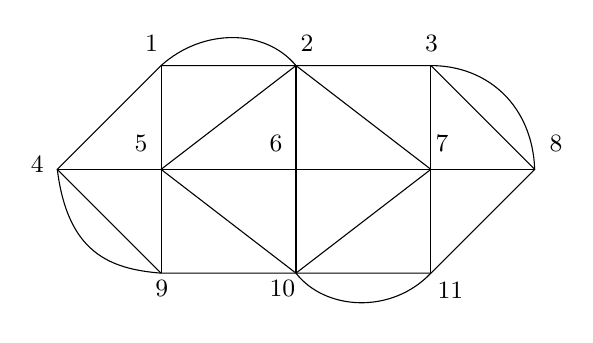
\begin{tikzpicture}[x=0.75pt,y=0.75pt,yscale=-1,xscale=1]
%uncomment if require: \path (0,341); %set diagram left start at 0, and has height of 341

%Shape: Polygon [id:ds4003763248080425] 
\draw   (80,30) -- (210,30) -- (260,80) -- (210,130) -- (80,130) -- (30,80) -- cycle ;
%Straight Lines [id:da24311625793640412] 
\draw    (80,130) -- (80,30) ;
%Straight Lines [id:da4577876944451016] 
\draw    (210,130) -- (210,30) ;
%Straight Lines [id:da21426374549674065] 
\draw    (145,130) -- (145,30) ;
%Straight Lines [id:da9411463237460063] 
\draw    (260,80) -- (30,80) ;
%Straight Lines [id:da6679107864804581] 
\draw    (80,80) -- (145,30) ;
%Straight Lines [id:da16808655880737433] 
\draw    (145,130) -- (210,80) ;
%Straight Lines [id:da5227136090162001] 
\draw    (80,80) -- (145,130) ;
%Straight Lines [id:da06804712905510657] 
\draw    (145,30) -- (210,80) ;
%Curve Lines [id:da028125126995495187] 
\draw    (80,30) .. controls (100,12) and (130,12) .. (145,30) ;
%Curve Lines [id:da2633729344718423] 
\draw    (30,80) .. controls (35,120) and (55,128) .. (80,130) ;
%Curve Lines [id:da8939842229082382] 
\draw    (210,30) .. controls (238,30) and (259,50) .. (260,80) ;
%Curve Lines [id:da7909135453505702] 
\draw    (145,130) .. controls (159,148) and (191,150) .. (210,130) ;

% Text Node
\draw (71,14.4) node [anchor=north west][inner sep=0.75pt]  [font=\small]  {$1$};
% Text Node
\draw (146,14.4) node [anchor=north west][inner sep=0.75pt]  [font=\small]  {$2$};
% Text Node
\draw (206,14.4) node [anchor=north west][inner sep=0.75pt]  [font=\small]  {$3$};
% Text Node
\draw (16,72.4) node [anchor=north west][inner sep=0.75pt]  [font=\small]  {$4$};
% Text Node
\draw (66,62.4) node [anchor=north west][inner sep=0.75pt]  [font=\small]  {$5$};
% Text Node
\draw (131,62.4) node [anchor=north west][inner sep=0.75pt]  [font=\small]  {$6$};
% Text Node
\draw (211,62.4) node [anchor=north west][inner sep=0.75pt]  [font=\small]  {$7$};
% Text Node
\draw (266,62.4) node [anchor=north west][inner sep=0.75pt]  [font=\small]  {$8$};
% Text Node
\draw (76,132.4) node [anchor=north west][inner sep=0.75pt]  [font=\small]  {$9$};
% Text Node
\draw (131,132.4) node [anchor=north west][inner sep=0.75pt]  [font=\small]  {$10$};
% Text Node
\draw (212,133.4) node [anchor=north west][inner sep=0.75pt]  [font=\small]  {$11$};

\end{tikzpicture}
\label{fig1}
\end{figure}

\section*{11.44}
By definition of bipartiteness, we may split the vertices into sets $V_m$, $V_n$. Further, each Hamiltonian path must alternate in vertices from $V_m$ and $V_n$. WLOG a Hamiltonian cycle must start in $V_m$ and end in $V_m$ so by parity $m = n$. A Hamiltonian path need not be so restricted, but since a vertex in one set cannot have a neighbor in the same set, we must have that $|m - n| \leq 1$ $\Box$

\section*{11.58}
First consider a graph with one connected component. By definition, a graph is a tree if and only if it has no cycles. Since cycles cannot span multiple connected components, a graph with arbitrarily many components has no cycles if and only if each component is a tree, that is, the graph is a forest $\Box$

\section*{11.63}
Possible spanning trees are marked with bold lines.
\begin{center}
\tikzset{every picture/.style={line width=0.75pt}} %set default line width to 0.75pt        
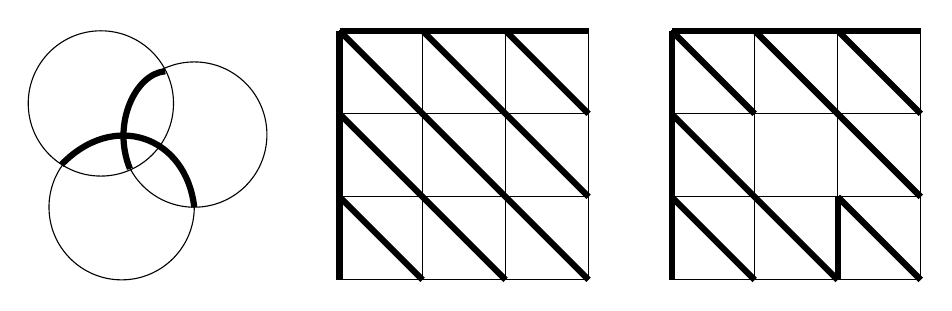
\begin{tikzpicture}[x=0.75pt,y=0.75pt,yscale=-1,xscale=1]
%uncomment if require: \path (0,341); %set diagram left start at 0, and has height of 341

%Shape: Circle [id:dp4961975584466247] 
\draw   (20,55) .. controls (20,35.67) and (35.67,20) .. (55,20) .. controls (74.33,20) and (90,35.67) .. (90,55) .. controls (90,74.33) and (74.33,90) .. (55,90) .. controls (35.67,90) and (20,74.33) .. (20,55) -- cycle ;
%Shape: Circle [id:dp6649724320953707] 
\draw   (30,105) .. controls (30,85.67) and (45.67,70) .. (65,70) .. controls (84.33,70) and (100,85.67) .. (100,105) .. controls (100,124.33) and (84.33,140) .. (65,140) .. controls (45.67,140) and (30,124.33) .. (30,105) -- cycle ;
%Shape: Circle [id:dp7220528696289328] 
\draw   (65,70) .. controls (65,50.67) and (80.67,35) .. (100,35) .. controls (119.33,35) and (135,50.67) .. (135,70) .. controls (135,89.33) and (119.33,105) .. (100,105) .. controls (80.67,105) and (65,89.33) .. (65,70) -- cycle ;
%Curve Lines [id:da9487111595253768] 
\draw [line width=2.25]    (36,84.5) .. controls (61,58.5) and (96,70.5) .. (100,105) ;
%Curve Lines [id:da9539790421576559] 
\draw [line width=2.25]    (69,86.5) .. controls (60,64.5) and (72,40.5) .. (86,39.5) ;
%Shape: Rectangle [id:dp051838398406386155] 
\draw   (170,20) -- (290,20) -- (290,140) -- (170,140) -- cycle ;
%Straight Lines [id:da8087311382253526] 
\draw    (170,60) -- (290,60) ;
%Straight Lines [id:da16332374711687914] 
\draw    (170,100) -- (290,100) ;
%Straight Lines [id:da25163039306599067] 
\draw    (210,20) -- (210,140) ;
%Straight Lines [id:da7387325487572696] 
\draw    (250,20) -- (250,140) ;
%Straight Lines [id:da18735282422681343] 
\draw [line width=2.25]    (250,20) -- (290,60) ;
%Straight Lines [id:da11311904038490384] 
\draw [line width=2.25]    (170,20) -- (290,140) ;
%Straight Lines [id:da2889395032290696] 
\draw [line width=2.25]    (210,20) -- (290,100) ;
%Straight Lines [id:da2875226416878216] 
\draw [line width=2.25]    (170,60) -- (250,140) ;
%Straight Lines [id:da636138659322756] 
\draw [line width=2.25]    (170,100) -- (210,140) ;
%Straight Lines [id:da9010818695021479] 
\draw [line width=2.25]    (170,20) -- (170,140) ;
%Straight Lines [id:da3624213198136652] 
\draw [line width=2.25]    (170,20) -- (290,20) ;
%Shape: Rectangle [id:dp38443682649392286] 
\draw   (330,20) -- (450,20) -- (450,140) -- (330,140) -- cycle ;
%Straight Lines [id:da46505500856729753] 
\draw    (330,60) -- (450,60) ;
%Straight Lines [id:da5852200392243554] 
\draw    (330,100) -- (450,100) ;
%Straight Lines [id:da2164771359936828] 
\draw    (370,20) -- (370,140) ;
%Straight Lines [id:da3351286609856463] 
\draw    (410,20) -- (410,140) ;
%Straight Lines [id:da935266322362353] 
\draw [line width=2.25]    (410,20) -- (450,60) ;
%Straight Lines [id:da5805920949481573] 
\draw [line width=2.25]    (370,20) -- (450,100) ;
%Straight Lines [id:da7069322045918749] 
\draw [line width=2.25]    (330,60) -- (410,140) ;
%Straight Lines [id:da8421633205148236] 
\draw [line width=2.25]    (330,100) -- (370,140) ;
%Straight Lines [id:da49341656136900336] 
\draw [line width=2.25]    (330,20) -- (330,140) ;
%Straight Lines [id:da6216470258888851] 
\draw [line width=2.25]    (330,20) -- (450,20) ;
%Straight Lines [id:da9501203729742389] 
\draw [line width=2.25]    (330,20) -- (370,60) ;
%Straight Lines [id:da7973502704352504] 
\draw [line width=2.25]    (410,100) -- (450,140) ;
%Straight Lines [id:da465848031597919] 
\draw [line width=2.25]    (410,100) -- (410,140) ;


\end{tikzpicture}
\end{center}

\section*{11.87a}
We prove by showing the minimal non-caterpillar tree contains 7 vertices. Consider arbitrary tree and fix path $\gamma = v_1, \dots, v_n$. The only way for this tree to not be a caterpillar is if there exists some subtree of depth at least 2 rooted at an internal vertex $v_i$, $i \neq 1, n$. The minimal way to form such a subtree is to have a simple internal \say{offshoot} of length 2. Label the vertices in this path $v_i, v_i^1, v_i^2$. Additionally, $i \neq 2, n-1$ since otherwise we could simply amend $\gamma$ to be $v_2^2, v_2^1, v_2, \dots, v_n$ and $v_1, \dots, v_{n-1}, v_{n-1}^1, v_{n-1}^2$ and the tree would again be a caterpillar. Then the minimal tree that is not a caterpillar is a tree with path $v_1, \dots, v_5$ and internal offshoot $v_3, v_3^1, v_3^2$. But this tree contains 7 vertices, so indeed all trees with 6 or fewer vertices are caterpillars $\Box$

\end{document}

% List of tex snippets:
%   - tex-header (this)
%   - R      --> \mathbb{R}
%   - Z      --> \mathbb{Z}
%   - B      --> \mathcal{B}
%   - E      --> \mathcal{E}
%   - M      --> \mathcal{M}
%   - m      --> \mathfrak{m}({#1})
%   - normlp --> \norm{{#1}}_{L^{{#2}}}
